\documentclass[12pt]{article}

\usepackage{sbc-template}

\usepackage{graphicx,url}

\usepackage[brazil]{babel}   
%\usepackage[latin1]{inputenc}  
\usepackage[utf8]{inputenc}  
% UTF-8 encoding is recommended by ShareLaTex

     
\sloppy

\title{Análisis, Estudio y Prototipo de un Conjunto de Servicios Web para recopilar datos de preguntas y respuestas médicas usando reconocimiento de Lenguaje Natural sobre un Sistema Cognitivo}

\author{Christian Guevara, Carolina López, Denisse Calle, Iván Carrera\inst{1}}


\address{Facultad de Ingenier{\'i}a de Sistemas -- Escuela Polit{\'e}cnica Nacional (EPN)\\
Ladr{\'o}n de Guevara E11-253. Quito -- Ecuador
\email{\{christian.guevara,carolina.lopez,ivan.carrera\}@epn.edu.ec, \newline denisse@hmedic.com}
}

\begin{document} 

\maketitle

\begin{abstract}
  
\end{abstract}
     
\begin{resumen} 
Este artículo describe un proyecto que usará un sistema cognitivo entrenado con información médica para responder inquietudes sobre prevención de la mortalidad materna utilizando un lenguaje natural. La información solicitada por el usuario y entregada por el sistema se almacena para un posterior análisis en el que, geolocalizando anónimamente a los usuarios, se buscarán factores que muestren un incremento en síntomas que afectan dentro de una zona geográfica. La información contribuirá con el Ministerio de Salud Pública del Ecuador para el programa de prevención de mortalidad materna y neonatal, y también con los objetivos del milenio planteados por la Organización Mundial de la Salud.
\end{resumen}


\section{Introducción}
Actualmente, los sistemas cognitivos pueden imitar las capacidades del cerebro humano \cite{banavar2015watson}, permitiendo que los computadores puedan analizar e interpretar información. % Sin embargo, no todas las personas tienen acceso a este tipo de sistemas, ya que se necesitan aplicaciones y conocimientos especializados en areas informaticas y de computación.
Uno de los sistemas cognitivos más utilizado en la actualidad es IBM Watson, disponible al público desde la plataforma IBM Bluemix \cite{watson2016}, en el que los usuarios pueden crear instancias para realizar análisis en temas específicos

Entre los servicios de Watson está \emph{Retrieve and Rank}, que recibe información estructurada para su procesamiento y posteriormente utilizada en el entrenamiento del modelo. El modelo de aprendizaje de este servicio se basa en un conjunto de preguntas, sus posibles respuestas y su respectivo nivel de asertividad. A través de dicho modelo se ofrecen los resultados mejor puntuados a las inquietudes planteadas por los usuarios \cite{watson2016}. 

El reto actual es lograr comunicación entre humano y computador a través de un lenguaje escrito y hablado por humanos, conocido como lenguaje natural \cite{ibm2015}, para ofrecer a los usuarios resultados acorde a sus necesidades, democratizando el acceso a la información médica existente.

El presente artículo propone la creación de una aplicación móvil que sea capaz de recibir preguntas médicas en lenguaje natural, a través de una interfaz fácil de usar que permita el ingreso de datos a través de un cuadro de texto o de una grabación de voz.% Al prototipo de la aplicación podrían tener acceso los usuarios que posean teléfonos inteligentes con acceso a internet.

Con la utilización de un conjunto de servicios web se recopilará la información anónima proveniente de las inquietudes de los usuarios ligada a la respuesta entregada por el sistema cognitivo. Dicha información servirá para un análisis posterior que permita determinar cuáles son las preguntas médicas y dudas más frecuentes durante el embarazo y primeros meses de vida del bebé, buscando disminuir el índice de mortalidad de madres y neonatos en el país.

En la Cumbre del Milenio realizada entre el 6 y 8 de septiembre de 2000, 189 países miembros de las Naciones Unidas firmaron la Declaración del Milenio, la misma que asume 8 Objetivos del Milenio como compromisos a cumplir hasta el 2015.

El Objetivo del Milenio (ODM) relacionado a la Salud Materna es el número 5: “Mejorar la Salud Materna”. El mismo tiene como una de sus metas reducir la Razón de Mortalidad Materna (RMM) en tres cuartas partes (75\%) entre 1990 y 2015.

La Organización Mundial de la Salud (OMS) define mortalidad materna al deceso de una mujer durante el embarazo, el parto o las 6 semanas después del parto.

Se reporta que el 99% de las muertes maternas corresponde a los países en desarrollo. Lo que se vincula directamente con el acceso a servicios de salud y cobertura universal. (OMS, 2015)

En el año 2015, Latinoamérica reportó 6000 muertes maternas. Lo que a su vez representa una Razón de Muerte Materna de 60. (OMS, 2015)

En Ecuador, desde 1990 se han establecido varios cambios en la política pública de salud, los mismos que han sido planteados con el objetivo de cumplir el compromiso de mejorar la salud materna.

Durante la década del los 90 el Ministerio de Salud Pública del Ecuador (MSP) creó la Ley de Maternidad Gratuita y Atención a la Infancia. En el año 2008 se publica el Plan Nacional de Reducción Acelerada de la Mortalidad Materna y Neonatal. Finalmente en el 2014, se implementa la Gerencia Institucional para la Reducción Acelerada de Muerte Materna. (MSP, 2015)

Los datos reportados (OMS, 2015), sobre el progreso de la disminución de la Muerte Materna en Ecuador, son los siguientes:


Tabla 1 Evolución de estimaciones de la razón de mortalidad materna en el período 1990-2015

Ecuador
	Razón de Muerte Materna	Cambio Porcentual de la RMM entre 1990-2015
	1990	1995	2000	2005	2010	2015	
	185	131	103	74	75	64	65,4
Nota: tomada de OMS (2015)

Ecuador ha logrado reducir la muerte materna en un 65,4%, lo que no llega a la meta establecida sin embargo muestra un evidente progreso en la Salud Materna Nacional.

La Norma para el Cuidado Obstétrico y Neonatal Esencia (CONE) en el Sistema Nacional de Salud, publicada en el 2013, reporta que el 55% de las causas de muerte materna pueden ser prevenibles.

“Otros factores que impiden que las mujeres reciban o busquen atención durante el embarazo y el parto son:
•	la pobreza;
•	la distancia;
•	la falta de información;
•	la inexistencia de servicios adecuados;
•	las prácticas culturales.

Para mejorar la salud materna hay que identificar y eliminar los obstáculos al acceso a servicios de salud materna de calidad en todos los niveles del sistema sanitario.” (OMS, 2015)

Carissa F. Etienne. Directora, Oficina Sanitaria Panamericana/Organización Panamericana de la Salud, Oficina Regional de la Organización Mundial de la Salud para las Américas (2014), menciona que:

Si se le da un buen uso y se aplica ampliamente, la eSalud puede ser una herramienta estratégica que permita mejorar el acceso, ampliar la cobertura y aumentar la eficiencia financiera de los sistemas de atención de salud. Las TIC ya están revolucionando el acceso a la atención integral de buena calidad, superando muchas dificultades y permitiendo que en la atención primaria se resuelvan más problemas de salud. Las TIC vinculan las redes integradas de atención, lo que permite derivaciones más rápidas y fáciles a los especialistas y los niveles secundarios de atención. Muchos otros usos se relacionan con los sistemas y registros de información sobre la salud, la capacitación y el aumento de la capacidad del personal de salud de primera línea, e incluso los mecanismos de rendición de cuentas.

En Ecuador, según cifras del Instituto Nacional de Estadística y Censos (INEC), la Encuesta de Condiciones de Vida del período 2013-2014 reporta que el 48,5% de ecuatorianos cuentan con una computadora/laptop y el 24,3% con un teléfono inteligente. 

Si a este dato le sumamos una aplicación móvil que permita realizar la captación y vigilancia en salud de las mujeres embarazadas que habitan en el Ecuador, podríamos prevenir sus muertes y de esa manera cumplir con el ahora Objetivo de Desarrollo Sostenible, que nace del Objetivo del Milenio, que ahora busca disminuir la RMM a 70 para el año 2030.

Para el 2015, la Mortalidad Materna disminuyó un 44\% desde 1990. (OMS, 2015)

\section{Diseño}
\label{sec:firstpage}

Para la construcción, alojamiento y ejecución de los diferentes componentes necesarios para el funcionamiento de la aplicación móvil, back-end y sistemas cognitivos se plantea el siguiente diagrama de arquitectura:

\begin{figure}[ht]
\centering
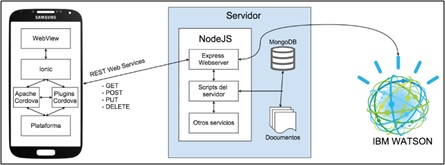
\includegraphics[width=.8\textwidth]{model.jpg}
\caption{Diagrama de Arquitectura}
\label{fig:exampleFig1}
\end{figure}

%\begin{figure}[ht]
%\centering
%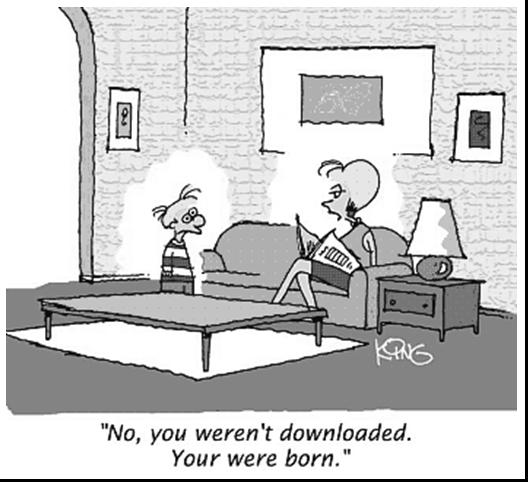
\includegraphics[width=.5\textwidth]{fig1.jpg}
%\caption{A typical figure}
%\label{fig:exampleFig1}
%\end{figure}
%
%\begin{figure}[ht]
%\centering
%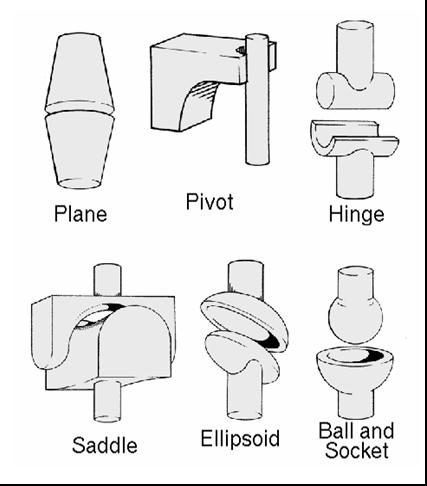
\includegraphics[width=.3\textwidth]{fig2.jpg}
%\caption{This figure is an example of a figure caption taking more than one
  %line and justified considering margins mentioned in Section~\ref{sec:figs}.}
%\label{fig:exampleFig2}
%\end{figure}

In tables, try to avoid the use of colored or shaded backgrounds, and avoid
thick, doubled, or unnecessary framing lines. When reporting empirical data,
do not use more decimal digits than warranted by their precision and
reproducibility. Table caption must be placed before the table (see Table 1)
and the font used must also be Helvetica, 10 point, boldface, with 6 points of
space before and after each caption.

\begin{table}[ht]
\centering
\caption{Variables to be considered on the evaluation of interaction
  techniques}
\label{tab:exTable1}
\smallskip
\begin{tabular}{|l|c|c|}
\hline
& Value 1 & Value 2\\[0.5ex]
\hline
&&\\[-2ex]
Case 1 & 1.0 $\pm$ 0.1 & 1.75$\times$10$^{-5}$ $\pm$ 5$\times$10$^{-7}$\\[0.5ex]
\hline
&&\\[-2ex]
Case 2 & 0.003(1) & 100.0\\[0.5ex]
\hline
\end{tabular}
\end{table}

\section{Images}

All images and illustrations should be in black-and-white, or gray tones,
excepting for the papers that will be electronically available (on CD-ROMs,
internet, etc.). The image resolution on paper should be about 600 dpi for
black-and-white images, and 150-300 dpi for grayscale images.  Do not include
images with excessive resolution, as they may take hours to print, without any
visible difference in the result. 

\section{References}

Bibliographic references must be unambiguous and uniform.  We recommend giving
the author names references in brackets, e.g. \cite{knuth:84},
\cite{boulic:91}, and \cite{smith:99}.

The references must be listed using 12 point font size, with 6 points of space
before each reference. The first line of each reference should not be
indented, while the subsequent should be indented by 0.5 cm.

\bibliographystyle{sbc}
\bibliography{sbc-template}

\end{document}
